\documentclass{beamer}

\usepackage[utf8]{inputenc}
\usepackage{listings}
\usepackage{tikz}
\usepackage{arrayjob}
\usepackage{amsmath}

\definecolor{mygreen}{rgb}{0,0.6,0}
\definecolor{mygray}{rgb}{0.5,0.5,0.5}
\definecolor{mymauve}{rgb}{0.58,0,0.82}


\usetikzlibrary{decorations.pathmorphing}

\tikzset{snake it/.style={decorate, decoration=snake}}

\lstset{ %
  backgroundcolor=\color{white},   % choose the background color; you must add \usepackage{color} or \usepackage{xcolor}
  basicstyle=\tiny,        % the size of the fonts that are used for the code
  breakatwhitespace=false,         % sets if automatic breaks should only happen at whitespace
  breaklines=true,                 % sets automatic line breaking
  commentstyle=\color{mygreen},    % comment style
  deletekeywords={...},            % if you want to delete keywords from the given language
  escapeinside={\%*}{*)},          % if you want to add LaTeX within your code
  extendedchars=true,              % lets you use non-ASCII characters; for 8-bits encodings only, does not work with UTF-8
  frame=single,                    % adds a frame around the code
  keepspaces=true,                 % keeps spaces in text, useful for keeping indentation of code (possibly needs columns=flexible)
  keywordstyle=\color{blue},       % keyword style
  language=Java,                 % the language of the code
  morekeywords={*,...},            % if you want to add more keywords to the set
  numbers=left,                    % where to put the line-numbers; possible values are (none, left, right)
  numbersep=5pt,                   % how far the line-numbers are from the code
  numberstyle=\tiny\color{mygray}, % the style that is used for the line-numbers
  rulecolor=\color{black},         % if not set, the frame-color may be changed on line-breaks within not-black text (e.g. comments (green here))
  showspaces=false,                % show spaces everywhere adding particular underscores; it overrides 'showstringspaces'
  showstringspaces=false,          % underline spaces within strings only
  showtabs=false,                  % show tabs within strings adding particular underscores
  stepnumber=1,                    % the step between two line-numbers. If it's 1, each line will be numbered
  stringstyle=\color{mymauve},     % string literal style
  tabsize=2                      % sets default tabsize to 2 spaces
}

\tikzstyle{vertex}=[circle,fill=gray!50,minimum size=15pt,inner sep=0pt]
\tikzstyle{visited}=[circle,fill=green!25,minimum size=15pt,inner sep=0pt]
\tikzstyle{unvisited}=[circle,fill=blue!25,minimum size=15pt,inner sep=0pt]


\tikzstyle{woman}=[circle,fill=pink!50,minimum size=15pt,inner sep=0pt]
\tikzstyle{men}=[circle,fill=blue!50,minimum size=15pt,inner sep=0pt]


\newcommand{\W}{\ {\color{red} \textbf{!!}} \ }

\begin{document}

\begin{frame}
\begin{center}
{\color{black} \huge{\textbf{Flows}}}
\end{center}
\end{frame}

\begin{frame}
	\begin{center}
		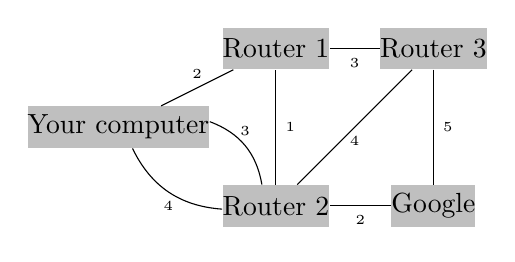
\begin{tikzpicture}
		\tikzstyle{vertex}=[rectangle,fill=gray!50,minimum size=15pt,inner sep=0pt]
		\node[vertex] at (0, 0) (s) {Your computer};
		\node[vertex] at (2, 1) (a) {Router 1};
		\node[vertex] at (2, -1) (b) {Router 2};
		\node[vertex] at (4, 1) (c) {Router 3};
		\node[vertex] at (4, -1) (t) {Google};
		\draw[-] (s) edge node[anchor = south] {\tiny $2$} (a);
		\draw[-] (s) edge[bend right] node[anchor = north] {\tiny $4$} (b);
		\draw[-] (a) edge node[anchor = north] {\tiny $3$} (c);
		\draw[-] (b) edge[bend right] node[anchor = south] {\tiny $3$} (s);
		\draw[-] (b) edge node[anchor = west] {\tiny $1$} (a);
		\draw[-] (c) edge node[anchor = north] {\tiny $4$} (b);
		\draw[-] (b) edge node[anchor = north] {\tiny $2$} (t);
		\draw[-] (c) edge node[anchor = west] {\tiny $5$} (t);
		\end{tikzpicture}
	\end{center}
	
\end{frame}

\begin{frame}[fragile]
	\begin{center}
		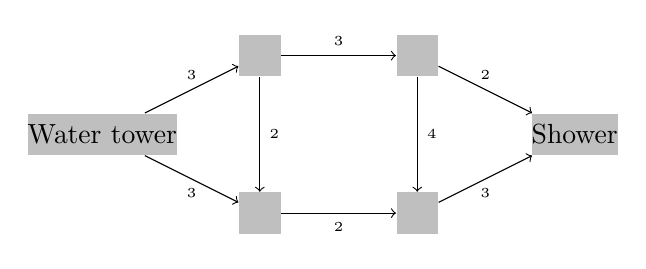
\begin{tikzpicture}
		\tikzstyle{vertex}=[rectangle,fill=gray!50,minimum size=15pt,inner sep=0pt]
		\node[vertex] (s) at (0, 0) {Water tower};
		\node[vertex] (o) at (2, 1) {$\ $};
		\node[vertex] (p) at (2, -1) {$\ $};
		\node[vertex] (q) at (4, 1) {$\ $};
		\node[vertex] (r) at (4, -1) {$\ $};
		\node[vertex] (t) at (6, 0) {Shower};
		
		\draw[->] (s) edge node[anchor = south] {\tiny $3$} (o);
		\draw[->] (o) edge node[anchor = south] (c) {\tiny $3$} (q);
		\draw[->] (q) edge node[anchor = south] {\tiny $2$} (t);
		\draw[->] (s) edge node[anchor = north] {\tiny $3$} (p);
		\draw[->] (o) edge node[anchor = west] {\tiny $2$} (p);
		\draw[->] (p) edge node[anchor = north] {\tiny $2$} (r);
		\draw[->] (q) edge node[anchor = west] {\tiny $4$} (r);
		\draw[->] (r) edge node[anchor = north] {\tiny $3$} (t);
		
		%\node[draw] (ls) at (-1, -1) {source};
		%\node[draw] (lt) at (7, 1) {sink};
		
		%\node[draw] (lc) at (3.2, 2.5) {edge capacity};
		
		%\node[draw] (lf) at (2.8, -2.5) {current flow};
		%\draw[dashed] (3.2, 1.6) -- (lc);
		%\draw[dashed] (2.8, -1.6) -- (lf);
		%\draw[dashed] (s) -- (ls);
		%\draw[dashed] (t) -- (lt);
		\end{tikzpicture}
	\end{center}
\end{frame}

\begin{frame}[fragile]

The \textbf{Maximum-flow} problem consists of finding the maximum amout of
information that can be transferred from a source node into a sink node in a graph.

\vspace{0.5cm}

Each edge has a \textbf{capacity}, this defines the maximum amount of 
information that can go through that edge.

\begin{center}
\includegraphics[scale=0.3]{capacity.jpg}
\end{center}

\end{frame}

\begin{frame}[fragile]
\begin{center}
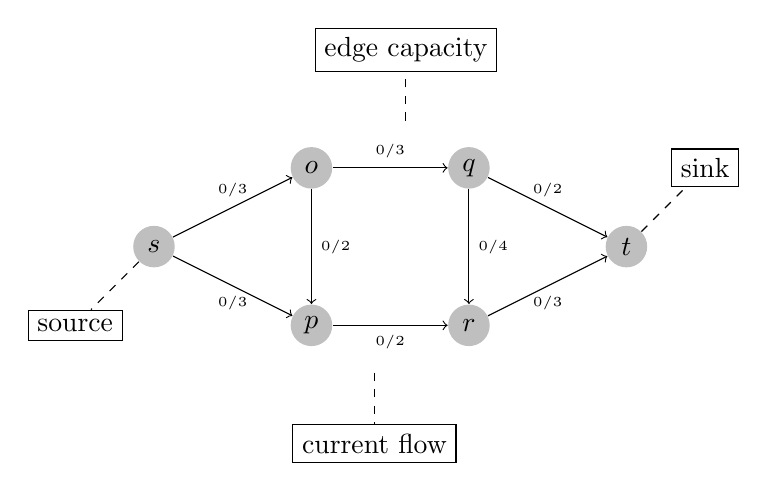
\begin{tikzpicture}
\node[vertex] (s) at (0, 0) {$s$};
\node[vertex] (o) at (2, 1) {$o$};
\node[vertex] (p) at (2, -1) {$p$};
\node[vertex] (q) at (4, 1) {$q$};
\node[vertex] (r) at (4, -1) {$r$};
\node[vertex] (t) at (6, 0) {$t$};

\draw[->] (s) edge node[anchor = south] {\tiny $0/3$} (o);
\draw[->] (o) edge node[anchor = south] (c) {\tiny $0/3$} (q);
\draw[->] (q) edge node[anchor = south] {\tiny $0/2$} (t);
\draw[->] (s) edge node[anchor = north] {\tiny $0/3$} (p);
\draw[->] (o) edge node[anchor = west] {\tiny $0/2$} (p);
\draw[->] (p) edge node[anchor = north] {\tiny $0/2$} (r);
\draw[->] (q) edge node[anchor = west] {\tiny $0/4$} (r);
\draw[->] (r) edge node[anchor = north] {\tiny $0/3$} (t);

\node[draw] (ls) at (-1, -1) {source};
\node[draw] (lt) at (7, 1) {sink};

\node[draw] (lc) at (3.2, 2.5) {edge capacity};

\node[draw] (lf) at (2.8, -2.5) {current flow};
\draw[dashed] (3.2, 1.6) -- (lc);
\draw[dashed] (2.8, -1.6) -- (lf);
\draw[dashed] (s) -- (ls);
\draw[dashed] (t) -- (lt);
\end{tikzpicture}
\end{center}
\end{frame}

\begin{frame}
\begin{center}
\includegraphics[scale = 0.5]{idea1.jpg} 
\end{center}
\end{frame}

\begin{frame}[fragile]
\begin{center}
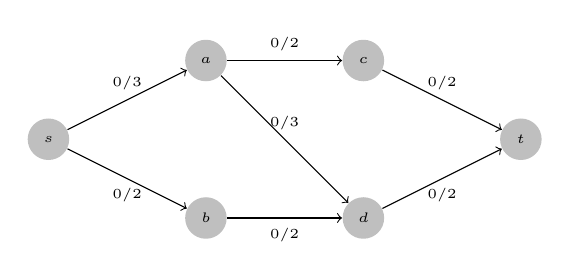
\begin{tikzpicture}
\node[vertex] at (0, 0) (s) {\tiny $s$};
\node[vertex] at (2, 1) (a) {\tiny $a$};
\node[vertex] at (2, -1) (b) {\tiny $b$};
\node[vertex] at (4, 1) (c) {\tiny $c$};
\node[vertex] at (4, -1) (d) {\tiny $d$};
\node[vertex] at (6, 0) (t) {\tiny $t$};
\draw[->] (s) edge node[anchor = south] {\tiny $0 / 3$} (a);
\draw[->] (s) edge node[anchor = north] {\tiny $0 / 2$} (b);
\draw[->] (a) edge node[anchor = south] {\tiny $0 / 2$} (c);
\draw[->] (a) edge node[anchor = south] {\tiny $0 / 3$} (d);
\draw[->] (b) edge node[anchor = north] {\tiny $0 / 2$} (d);
\draw[->] (c) edge node[anchor = south] {\tiny $0 / 2$} (t);
\draw[->] (d) edge node[anchor = north] {\tiny $0 / 2$} (t);
\end{tikzpicture}
\end{center}
\end{frame}

\begin{frame}[fragile]
\begin{center}
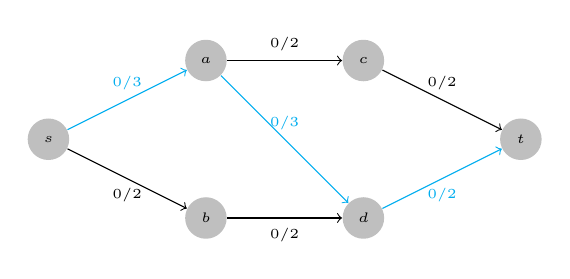
\begin{tikzpicture}
\node[vertex] at (0, 0) (s) {\tiny $s$};
\node[vertex] at (2, 1) (a) {\tiny $a$};
\node[vertex] at (2, -1) (b) {\tiny $b$};
\node[vertex] at (4, 1) (c) {\tiny $c$};
\node[vertex] at (4, -1) (d) {\tiny $d$};
\node[vertex] at (6, 0) (t) {\tiny $t$};
\draw[->, cyan] (s) edge node[anchor = south] {\tiny $0 / 3$} (a);
\draw[->] (s) edge node[anchor = north] {\tiny $0 / 2$} (b);
\draw[->] (a) edge node[anchor = south] {\tiny $0 / 2$} (c);
\draw[->, cyan] (a) edge node[anchor = south] {\tiny $0 / 3$} (d);
\draw[->] (b) edge node[anchor = north] {\tiny $0 / 2$} (d);
\draw[->] (c) edge node[anchor = south] {\tiny $0 / 2$} (t);
\draw[->, cyan] (d) edge node[anchor = north] {\tiny $0 / 2$} (t);
\end{tikzpicture}
\end{center}
\end{frame}

\begin{frame}[fragile]
\begin{center}
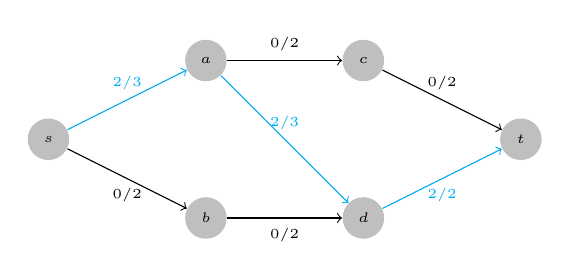
\begin{tikzpicture}
\node[vertex] at (0, 0) (s) {\tiny $s$};
\node[vertex] at (2, 1) (a) {\tiny $a$};
\node[vertex] at (2, -1) (b) {\tiny $b$};
\node[vertex] at (4, 1) (c) {\tiny $c$};
\node[vertex] at (4, -1) (d) {\tiny $d$};
\node[vertex] at (6, 0) (t) {\tiny $t$};
\draw[->, cyan] (s) edge node[anchor = south] {\tiny $2 / 3$} (a);
\draw[->] (s) edge node[anchor = north] {\tiny $0 / 2$} (b);
\draw[->] (a) edge node[anchor = south] {\tiny $0 / 2$} (c);
\draw[->, cyan] (a) edge node[anchor = south] {\tiny $2 / 3$} (d);
\draw[->] (b) edge node[anchor = north] {\tiny $0 / 2$} (d);
\draw[->] (c) edge node[anchor = south] {\tiny $0 / 2$} (t);
\draw[->, cyan] (d) edge node[anchor = north] {\tiny $2 / 2$} (t);
\end{tikzpicture}
\end{center}
\end{frame}

\begin{frame}[fragile]
\begin{center}
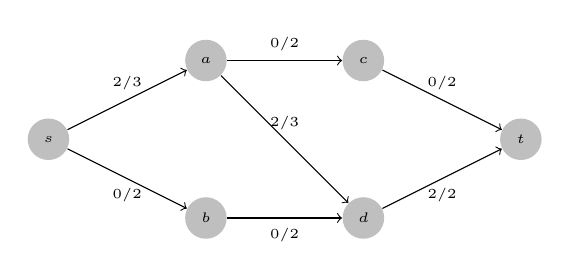
\begin{tikzpicture}
\node[vertex] at (0, 0) (s) {\tiny $s$};
\node[vertex] at (2, 1) (a) {\tiny $a$};
\node[vertex] at (2, -1) (b) {\tiny $b$};
\node[vertex] at (4, 1) (c) {\tiny $c$};
\node[vertex] at (4, -1) (d) {\tiny $d$};
\node[vertex] at (6, 0) (t) {\tiny $t$};
\draw[->] (s) edge node[anchor = south] {\tiny $2 / 3$} (a);
\draw[->] (s) edge node[anchor = north] {\tiny $0 / 2$} (b);
\draw[->] (a) edge node[anchor = south] {\tiny $0 / 2$} (c);
\draw[->] (a) edge node[anchor = south] {\tiny $2 / 3$} (d);
\draw[->] (b) edge node[anchor = north] {\tiny $0 / 2$} (d);
\draw[->] (c) edge node[anchor = south] {\tiny $0 / 2$} (t);
\draw[->] (d) edge node[anchor = north] {\tiny $2 / 2$} (t);
\end{tikzpicture}
\end{center}
\end{frame}

\begin{frame}[fragile]
\begin{center}
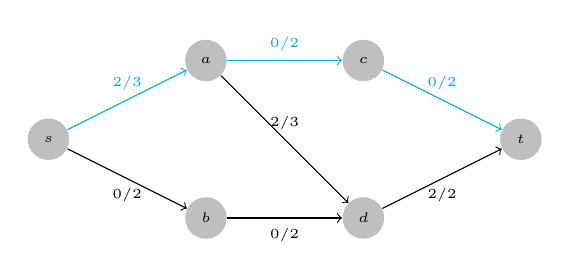
\begin{tikzpicture}
\node[vertex] at (0, 0) (s) {\tiny $s$};
\node[vertex] at (2, 1) (a) {\tiny $a$};
\node[vertex] at (2, -1) (b) {\tiny $b$};
\node[vertex] at (4, 1) (c) {\tiny $c$};
\node[vertex] at (4, -1) (d) {\tiny $d$};
\node[vertex] at (6, 0) (t) {\tiny $t$};
\draw[->, cyan] (s) edge node[anchor = south] {\tiny $2 / 3$} (a);
\draw[->] (s) edge node[anchor = north] {\tiny $0 / 2$} (b);
\draw[->, cyan] (a) edge node[anchor = south] {\tiny $0 / 2$} (c);
\draw[->] (a) edge node[anchor = south] {\tiny $2 / 3$} (d);
\draw[->] (b) edge node[anchor = north] {\tiny $0 / 2$} (d);
\draw[->, cyan] (c) edge node[anchor = south] {\tiny $0 / 2$} (t);
\draw[->] (d) edge node[anchor = north] {\tiny $2 / 2$} (t);
\end{tikzpicture}
\end{center}
\end{frame}

\begin{frame}[fragile]
\begin{center}
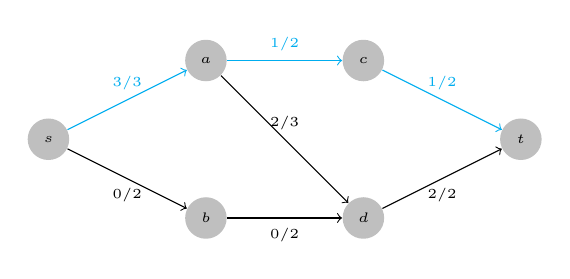
\begin{tikzpicture}
\node[vertex] at (0, 0) (s) {\tiny $s$};
\node[vertex] at (2, 1) (a) {\tiny $a$};
\node[vertex] at (2, -1) (b) {\tiny $b$};
\node[vertex] at (4, 1) (c) {\tiny $c$};
\node[vertex] at (4, -1) (d) {\tiny $d$};
\node[vertex] at (6, 0) (t) {\tiny $t$};
\draw[->, cyan] (s) edge node[anchor = south] {\tiny $3 / 3$} (a);
\draw[->] (s) edge node[anchor = north] {\tiny $0 / 2$} (b);
\draw[->, cyan] (a) edge node[anchor = south] {\tiny $1 / 2$} (c);
\draw[->] (a) edge node[anchor = south] {\tiny $2 / 3$} (d);
\draw[->] (b) edge node[anchor = north] {\tiny $0 / 2$} (d);
\draw[->, cyan] (c) edge node[anchor = south] {\tiny $1 / 2$} (t);
\draw[->] (d) edge node[anchor = north] {\tiny $2 / 2$} (t);
\end{tikzpicture}
\end{center}
\end{frame}

\begin{frame}[fragile]
\begin{center}
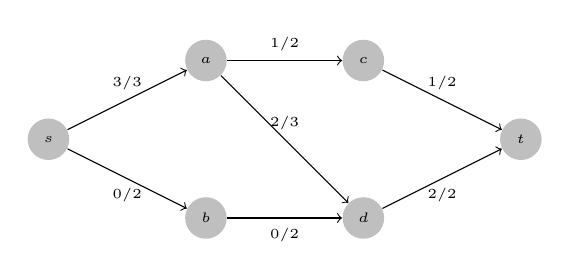
\begin{tikzpicture}
\node[vertex] at (0, 0) (s) {\tiny $s$};
\node[vertex] at (2, 1) (a) {\tiny $a$};
\node[vertex] at (2, -1) (b) {\tiny $b$};
\node[vertex] at (4, 1) (c) {\tiny $c$};
\node[vertex] at (4, -1) (d) {\tiny $d$};
\node[vertex] at (6, 0) (t) {\tiny $t$};
\draw[->] (s) edge node[anchor = south] {\tiny $3 / 3$} (a);
\draw[->] (s) edge node[anchor = north] {\tiny $0 / 2$} (b);
\draw[->] (a) edge node[anchor = south] {\tiny $1 / 2$} (c);
\draw[->] (a) edge node[anchor = south] {\tiny $2 / 3$} (d);
\draw[->] (b) edge node[anchor = north] {\tiny $0 / 2$} (d);
\draw[->] (c) edge node[anchor = south] {\tiny $1 / 2$} (t);
\draw[->] (d) edge node[anchor = north] {\tiny $2 / 2$} (t);
\end{tikzpicture}
\end{center}
\end{frame}


\begin{frame}[fragile]
\begin{center}
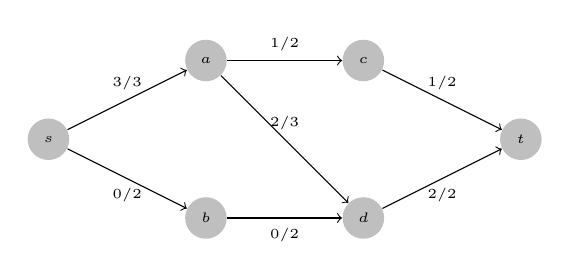
\begin{tikzpicture}
\node[vertex] at (0, 0) (s) {\tiny $s$};
\node[vertex] at (2, 1) (a) {\tiny $a$};
\node[vertex] at (2, -1) (b) {\tiny $b$};
\node[vertex] at (4, 1) (c) {\tiny $c$};
\node[vertex] at (4, -1) (d) {\tiny $d$};
\node[vertex] at (6, 0) (t) {\tiny $t$};
\draw[->] (s) edge node[anchor = south] {\tiny $3 / 3$} (a);
\draw[->] (s) edge node[anchor = north] {\tiny $0 / 2$} (b);
\draw[->] (a) edge node[anchor = south] {\tiny $1 / 2$} (c);
\draw[->] (a) edge node[anchor = south] {\tiny $2 / 3$} (d);
\draw[->] (b) edge node[anchor = north] {\tiny $0 / 2$} (d);
\draw[->] (c) edge node[anchor = south] {\tiny $1 / 2$} (t);
\draw[->] (d) edge node[anchor = north] {\tiny $2 / 2$} (t);
\end{tikzpicture}
\end{center}

No more paths. Found flow of value $3$. \textbf{Not} optimal!

\pause

\begin{center}
\includegraphics[scale = 0.18]{bad.jpg} 
\end{center}

We would like to be able to reconsider decisions.

\end{frame}

\begin{frame}[fragile]
\begin{center}
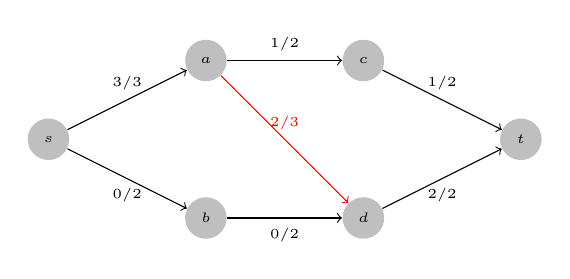
\begin{tikzpicture}
\node[vertex] at (0, 0) (s) {\tiny $s$};
\node[vertex] at (2, 1) (a) {\tiny $a$};
\node[vertex] at (2, -1) (b) {\tiny $b$};
\node[vertex] at (4, 1) (c) {\tiny $c$};
\node[vertex] at (4, -1) (d) {\tiny $d$};
\node[vertex] at (6, 0) (t) {\tiny $t$};
\draw[->] (s) edge node[anchor = south] {\tiny $3 / 3$} (a);
\draw[->] (s) edge node[anchor = north] {\tiny $0 / 2$} (b);
\draw[->] (a) edge node[anchor = south] {\tiny $1 / 2$} (c);
\draw[->, red] (a) edge node[anchor = south] {\tiny $2 / 3$} (d);
\draw[->] (b) edge node[anchor = north] {\tiny $0 / 2$} (d);
\draw[->] (c) edge node[anchor = south] {\tiny $1 / 2$} (t);
\draw[->] (d) edge node[anchor = north] {\tiny $2 / 2$} (t);
\end{tikzpicture}
\end{center}

\end{frame}

\begin{frame}[fragile]
\begin{center}
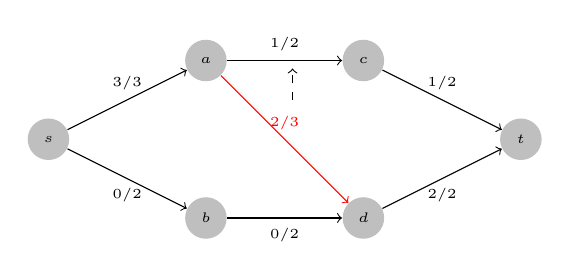
\begin{tikzpicture}
\node[vertex] at (0, 0) (s) {\tiny $s$};
\node[vertex] at (2, 1) (a) {\tiny $a$};
\node[vertex] at (2, -1) (b) {\tiny $b$};
\node[vertex] at (4, 1) (c) {\tiny $c$};
\node[vertex] at (4, -1) (d) {\tiny $d$};
\node[vertex] at (6, 0) (t) {\tiny $t$};
\draw[->] (s) edge node[anchor = south] {\tiny $3 / 3$} (a);
\draw[->] (s) edge node[anchor = north] {\tiny $0 / 2$} (b);
\draw[->] (a) edge node[anchor = south] {\tiny $1 / 2$} (c);
\draw[->, red] (a) edge node[anchor = south] {\tiny $2 / 3$} (d);
\draw[->] (b) edge node[anchor = north] {\tiny $0 / 2$} (d);
\draw[->] (c) edge node[anchor = south] {\tiny $1 / 2$} (t);
\draw[->] (d) edge node[anchor = north] {\tiny $2 / 2$} (t);

\draw[->, dashed] (3.1, 0.5) -- (3.1, 0.9);

\end{tikzpicture}
\end{center}

\end{frame}

\begin{frame}[fragile]
\begin{center}
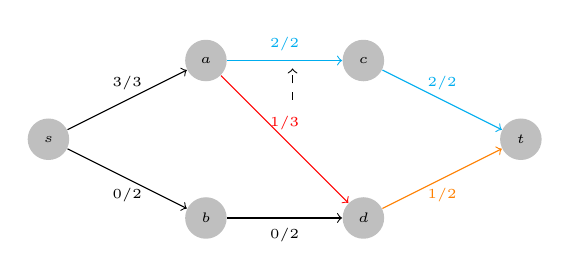
\begin{tikzpicture}
\node[vertex] at (0, 0) (s) {\tiny $s$};
\node[vertex] at (2, 1) (a) {\tiny $a$};
\node[vertex] at (2, -1) (b) {\tiny $b$};
\node[vertex] at (4, 1) (c) {\tiny $c$};
\node[vertex] at (4, -1) (d) {\tiny $d$};
\node[vertex] at (6, 0) (t) {\tiny $t$};
\draw[->] (s) edge node[anchor = south] {\tiny $3 / 3$} (a);
\draw[->] (s) edge node[anchor = north] {\tiny $0 / 2$} (b);
\draw[->, cyan] (a) edge node[anchor = south] {\tiny $2 / 2$} (c);
\draw[->, red] (a) edge node[anchor = south] {\tiny $1 / 3$} (d);
\draw[->] (b) edge node[anchor = north] {\tiny $0 / 2$} (d);
\draw[->, cyan] (c) edge node[anchor = south] {\tiny $2 / 2$} (t);
\draw[->, orange] (d) edge node[anchor = north] {\tiny $1 / 2$} (t);

\draw[->, dashed] (3.1, 0.5) -- (3.1, 0.9);

\end{tikzpicture}
\end{center}

\end{frame}

\begin{frame}[fragile]
\begin{center}
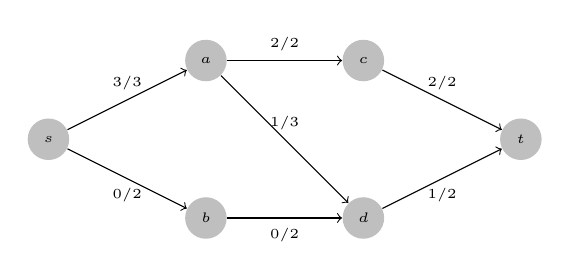
\begin{tikzpicture}
\node[vertex] at (0, 0) (s) {\tiny $s$};
\node[vertex] at (2, 1) (a) {\tiny $a$};
\node[vertex] at (2, -1) (b) {\tiny $b$};
\node[vertex] at (4, 1) (c) {\tiny $c$};
\node[vertex] at (4, -1) (d) {\tiny $d$};
\node[vertex] at (6, 0) (t) {\tiny $t$};
\draw[->] (s) edge node[anchor = south] {\tiny $3 / 3$} (a);
\draw[->] (s) edge node[anchor = north] {\tiny $0 / 2$} (b);
\draw[->] (a) edge node[anchor = south] {\tiny $2 / 2$} (c);
\draw[->] (a) edge node[anchor = south] {\tiny $1 / 3$} (d);
\draw[->] (b) edge node[anchor = north] {\tiny $0 / 2$} (d);
\draw[->] (c) edge node[anchor = south] {\tiny $2 / 2$} (t);
\draw[->] (d) edge node[anchor = north] {\tiny $1 / 2$} (t);
\end{tikzpicture}
\end{center}

\end{frame}

\begin{frame}[fragile]
\begin{center}
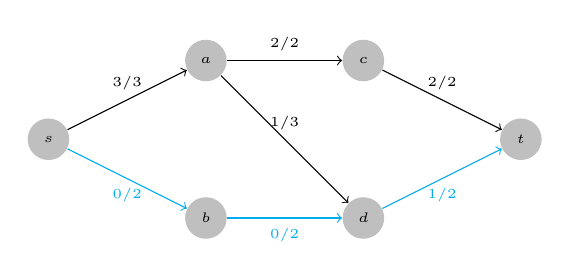
\begin{tikzpicture}
\node[vertex] at (0, 0) (s) {\tiny $s$};
\node[vertex] at (2, 1) (a) {\tiny $a$};
\node[vertex] at (2, -1) (b) {\tiny $b$};
\node[vertex] at (4, 1) (c) {\tiny $c$};
\node[vertex] at (4, -1) (d) {\tiny $d$};
\node[vertex] at (6, 0) (t) {\tiny $t$};
\draw[->] (s) edge node[anchor = south] {\tiny $3 / 3$} (a);
\draw[->, cyan] (s) edge node[anchor = north] {\tiny $0 / 2$} (b);
\draw[->] (a) edge node[anchor = south] {\tiny $2 / 2$} (c);
\draw[->] (a) edge node[anchor = south] {\tiny $1 / 3$} (d);
\draw[->, cyan] (b) edge node[anchor = north] {\tiny $0 / 2$} (d);
\draw[->] (c) edge node[anchor = south] {\tiny $2 / 2$} (t);
\draw[->, cyan] (d) edge node[anchor = north] {\tiny $1 / 2$} (t);
\end{tikzpicture}
\end{center}

\end{frame}


\begin{frame}[fragile]
\begin{center}
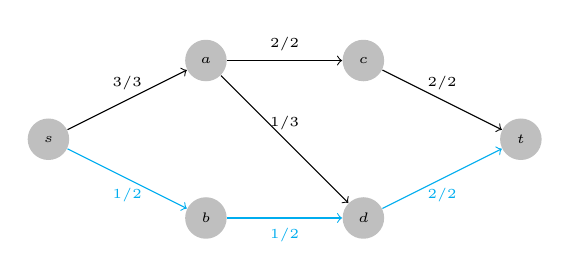
\begin{tikzpicture}
\node[vertex] at (0, 0) (s) {\tiny $s$};
\node[vertex] at (2, 1) (a) {\tiny $a$};
\node[vertex] at (2, -1) (b) {\tiny $b$};
\node[vertex] at (4, 1) (c) {\tiny $c$};
\node[vertex] at (4, -1) (d) {\tiny $d$};
\node[vertex] at (6, 0) (t) {\tiny $t$};
\draw[->] (s) edge node[anchor = south] {\tiny $3 / 3$} (a);
\draw[->, cyan] (s) edge node[anchor = north] {\tiny $1 / 2$} (b);
\draw[->] (a) edge node[anchor = south] {\tiny $2 / 2$} (c);
\draw[->] (a) edge node[anchor = south] {\tiny $1 / 3$} (d);
\draw[->, cyan] (b) edge node[anchor = north] {\tiny $1 / 2$} (d);
\draw[->] (c) edge node[anchor = south] {\tiny $2 / 2$} (t);
\draw[->, cyan] (d) edge node[anchor = north] {\tiny $2 / 2$} (t);
\end{tikzpicture}
\end{center}

\end{frame}

\begin{frame}[fragile]
\begin{center}
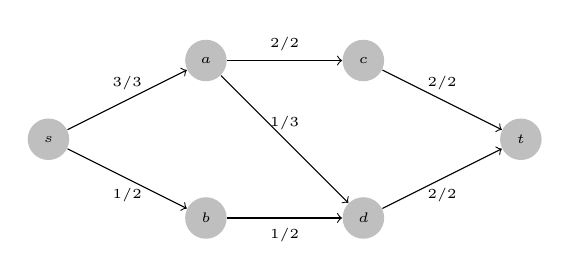
\begin{tikzpicture}
\node[vertex] at (0, 0) (s) {\tiny $s$};
\node[vertex] at (2, 1) (a) {\tiny $a$};
\node[vertex] at (2, -1) (b) {\tiny $b$};
\node[vertex] at (4, 1) (c) {\tiny $c$};
\node[vertex] at (4, -1) (d) {\tiny $d$};
\node[vertex] at (6, 0) (t) {\tiny $t$};
\draw[->] (s) edge node[anchor = south] {\tiny $3 / 3$} (a);
\draw[->] (s) edge node[anchor = north] {\tiny $1 / 2$} (b);
\draw[->] (a) edge node[anchor = south] {\tiny $2 / 2$} (c);
\draw[->] (a) edge node[anchor = south] {\tiny $1 / 3$} (d);
\draw[->] (b) edge node[anchor = north] {\tiny $1 / 2$} (d);
\draw[->] (c) edge node[anchor = south] {\tiny $2 / 2$} (t);
\draw[->] (d) edge node[anchor = north] {\tiny $2 / 2$} (t);
\end{tikzpicture}
\end{center}

\begin{itemize}
 \item No more paths. Found flow of value $4$. Optimal!
\end{itemize}
\end{frame}

\begin{frame}[fragile]
What we did corresponds to pushing flow on the following path:
\begin{center}
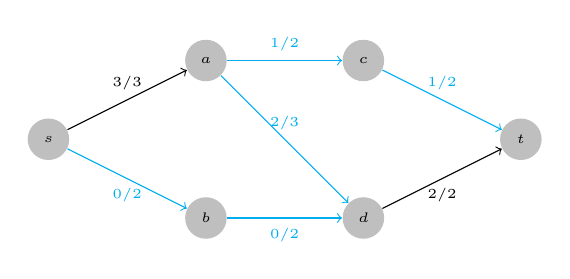
\begin{tikzpicture}
\node[vertex] at (0, 0) (s) {\tiny $s$};
\node[vertex] at (2, 1) (a) {\tiny $a$};
\node[vertex] at (2, -1) (b) {\tiny $b$};
\node[vertex] at (4, 1) (c) {\tiny $c$};
\node[vertex] at (4, -1) (d) {\tiny $d$};
\node[vertex] at (6, 0) (t) {\tiny $t$};
\draw[->] (s) edge node[anchor = south] {\tiny $3 / 3$} (a);
\draw[->, cyan] (s) edge node[anchor = north] {\tiny $0 / 2$} (b);
\draw[->, cyan] (a) edge node[anchor = south] {\tiny $1 / 2$} (c);
\draw[->, cyan] (a) edge node[anchor = south] {\tiny $2 / 3$} (d);
\draw[->, cyan] (b) edge node[anchor = north] {\tiny $0 / 2$} (d);
\draw[->, cyan] (c) edge node[anchor = south] {\tiny $1 / 2$} (t);
\draw[->] (d) edge node[anchor = north] {\tiny $2 / 2$} (t);
\end{tikzpicture}
\end{center}

\end{frame}

\begin{frame}[fragile]
What we did corresponds to pushing flow on the following path:
\begin{center}
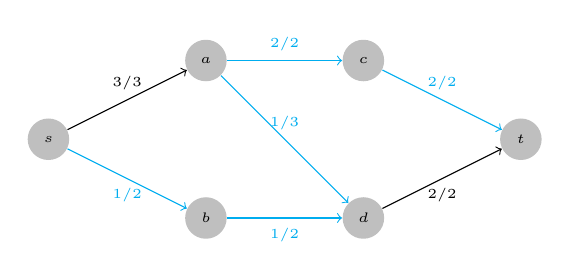
\begin{tikzpicture}
\node[vertex] at (0, 0) (s) {\tiny $s$};
\node[vertex] at (2, 1) (a) {\tiny $a$};
\node[vertex] at (2, -1) (b) {\tiny $b$};
\node[vertex] at (4, 1) (c) {\tiny $c$};
\node[vertex] at (4, -1) (d) {\tiny $d$};
\node[vertex] at (6, 0) (t) {\tiny $t$};
\draw[->] (s) edge node[anchor = south] {\tiny $3 / 3$} (a);
\draw[->, cyan] (s) edge node[anchor = north] {\tiny $1 / 2$} (b);
\draw[->, cyan] (a) edge node[anchor = south] {\tiny $2 / 2$} (c);
\draw[->, cyan] (a) edge node[anchor = south] {\tiny $1 / 3$} (d);
\draw[->, cyan] (b) edge node[anchor = north] {\tiny $1 / 2$} (d);
\draw[->, cyan] (c) edge node[anchor = south] {\tiny $2 / 2$} (t);
\draw[->] (d) edge node[anchor = north] {\tiny $2 / 2$} (t);
\end{tikzpicture}
\end{center}

\end{frame}


\begin{frame}[fragile]
What we did corresponds to pushing flow on the following path:
\begin{center}
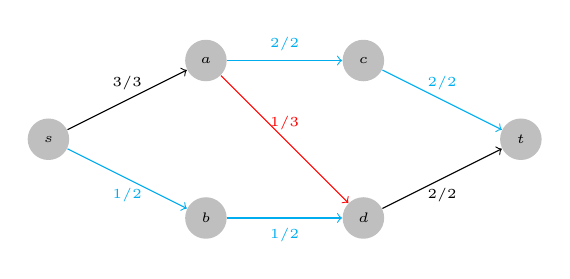
\begin{tikzpicture}
\node[vertex] at (0, 0) (s) {\tiny $s$};
\node[vertex] at (2, 1) (a) {\tiny $a$};
\node[vertex] at (2, -1) (b) {\tiny $b$};
\node[vertex] at (4, 1) (c) {\tiny $c$};
\node[vertex] at (4, -1) (d) {\tiny $d$};
\node[vertex] at (6, 0) (t) {\tiny $t$};
\draw[->] (s) edge node[anchor = south] {\tiny $3 / 3$} (a);
\draw[->, cyan] (s) edge node[anchor = north] {\tiny $1 / 2$} (b);
\draw[->, cyan] (a) edge node[anchor = south] {\tiny $2 / 2$} (c);
\draw[->, red] (a) edge node[anchor = south] {\tiny $1 / 3$} (d);
\draw[->, cyan] (b) edge node[anchor = north] {\tiny $1 / 2$} (d);
\draw[->, cyan] (c) edge node[anchor = south] {\tiny $2 / 2$} (t);
\draw[->] (d) edge node[anchor = north] {\tiny $2 / 2$} (t);
\end{tikzpicture}
\end{center}

\begin{center}
\includegraphics[scale = 0.25]{reverse.jpg}
\end{center}

\end{frame}

\begin{frame}[fragile]
This leads to the definition of \textbf{residual graph}.

\vspace{1cm}

Original

\begin{center}
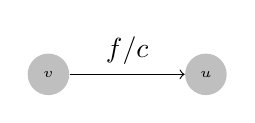
\begin{tikzpicture}
\node[vertex] at (0, 0) (v) {\tiny $v$};
\node[vertex] at (2, 0) (u) {\tiny $u$};
\draw[->] (v) edge node[anchor = south] {$f / c$} (u);
\end{tikzpicture}
\end{center}

\vspace{1cm}

Residual

\begin{center}
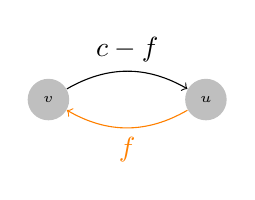
\begin{tikzpicture}
\node[vertex] at (0, 0) (v) {\tiny $v$};
\node[vertex] at (2, 0) (u) {\tiny $u$};
\draw[->] (v) edge[bend left] node[anchor = south] {$c - f$} (u);
\draw[<-, orange] (v) edge[bend right] node[anchor = north] {$f$} (u);
\end{tikzpicture}
\end{center}

\end{frame}

\begin{frame}

\begin{center}
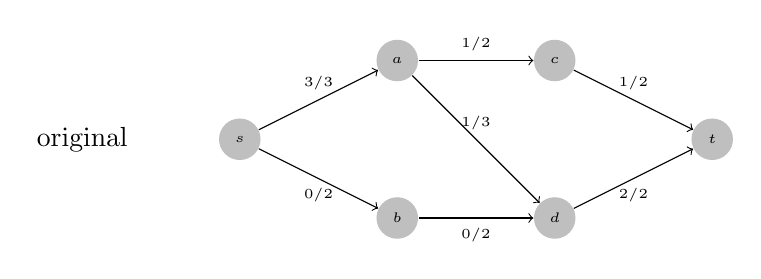
\begin{tikzpicture}
\node[vertex] at (0, 0) (s) {\tiny $s$};
\node[vertex] at (2, 1) (a) {\tiny $a$};
\node[vertex] at (2, -1) (b) {\tiny $b$};
\node[vertex] at (4, 1) (c) {\tiny $c$};
\node[vertex] at (4, -1) (d) {\tiny $d$};
\node[vertex] at (6, 0) (t) {\tiny $t$};
\draw[->] (s) edge node[anchor = south] {\tiny $3 / 3$} (a);
\draw[->] (s) edge node[anchor = north] {\tiny $0 / 2$} (b);
\draw[->] (a) edge node[anchor = south] {\tiny $1 / 2$} (c);
\draw[->] (a) edge node[anchor = south] {\tiny $1 / 3$} (d);
\draw[->] (b) edge node[anchor = north] {\tiny $0 / 2$} (d);
\draw[->] (c) edge node[anchor = south] {\tiny $1 / 2$} (t);
\draw[->] (d) edge node[anchor = north] {\tiny $2 / 2$} (t);
\node at (-2, 0) {original};
\end{tikzpicture}
\end{center}

\begin{center}
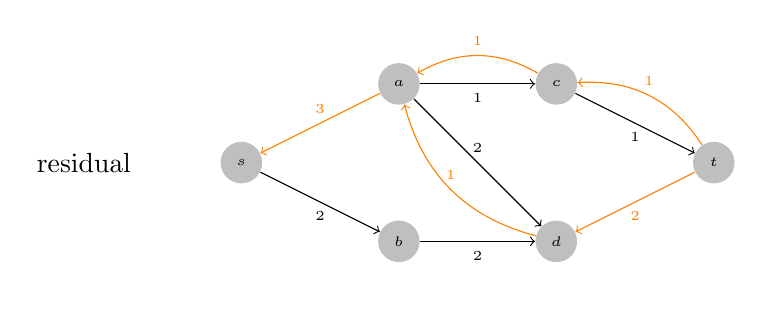
\begin{tikzpicture}
\node[vertex] at (0, 0) (s) {\tiny $s$};
\node[vertex] at (2, 1) (a) {\tiny $a$};
\node[vertex] at (2, -1) (b) {\tiny $b$};
\node[vertex] at (4, 1) (c) {\tiny $c$};
\node[vertex] at (4, -1) (d) {\tiny $d$};
\node[vertex] at (6, 0) (t) {\tiny $t$};
\draw[<-, orange] (s) edge node[anchor = south] {\tiny $3$} (a);
\draw[->] (s) edge node[anchor = north] {\tiny $2$} (b);
\draw[->] (a) edge node[anchor = north] {\tiny $1$} (c);
\draw[<-, orange] (a) edge[bend left] node[anchor = south] {\tiny $1$} (c);
\draw[<-, orange] (a) edge[bend right] node[anchor = south] {\tiny $1$} (d);
\draw[->] (a) edge node[anchor = south] {\tiny $2$} (d);
\draw[->] (b) edge node[anchor = north] {\tiny $2$} (d);
\draw[<-, orange] (c) edge[bend left] node[anchor = south] {\tiny $1$} (t);
\draw[->] (c) edge node[anchor = north] {\tiny $1$} (t);
\draw[<-, orange] (d) edge node[anchor = north] {\tiny $2$} (t);
\draw[<-, white] (s) edge[bend right] node[anchor = north] {\tiny $1$} (b);
\draw[<-, white] (b) edge[bend right] node[anchor = north] {\tiny $1$} (d);

\node at (-2, 0) {residual};
\end{tikzpicture}
\end{center}
\end{frame}


\begin{frame} 
\begin{center}
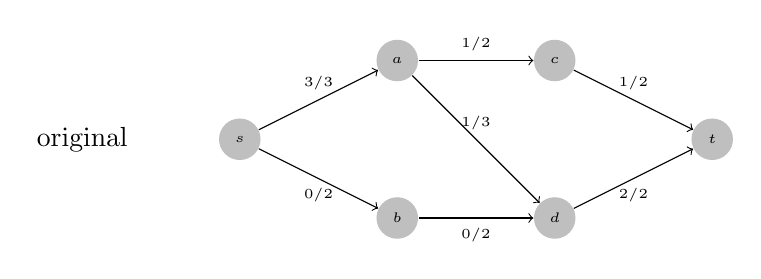
\begin{tikzpicture}
\node[vertex] at (0, 0) (s) {\tiny $s$};
\node[vertex] at (2, 1) (a) {\tiny $a$};
\node[vertex] at (2, -1) (b) {\tiny $b$};
\node[vertex] at (4, 1) (c) {\tiny $c$};
\node[vertex] at (4, -1) (d) {\tiny $d$};
\node[vertex] at (6, 0) (t) {\tiny $t$};
\draw[->] (s) edge node[anchor = south] {\tiny $3 / 3$} (a);
\draw[->] (s) edge node[anchor = north] {\tiny $0 / 2$} (b);
\draw[->] (a) edge node[anchor = south] {\tiny $1 / 2$} (c);
\draw[->] (a) edge node[anchor = south] {\tiny $1 / 3$} (d);
\draw[->] (b) edge node[anchor = north] {\tiny $0 / 2$} (d);
\draw[->] (c) edge node[anchor = south] {\tiny $1 / 2$} (t);
\draw[->] (d) edge node[anchor = north] {\tiny $2 / 2$} (t);
\node at (-2, 0) {original};
\end{tikzpicture}
\end{center}

\begin{center}
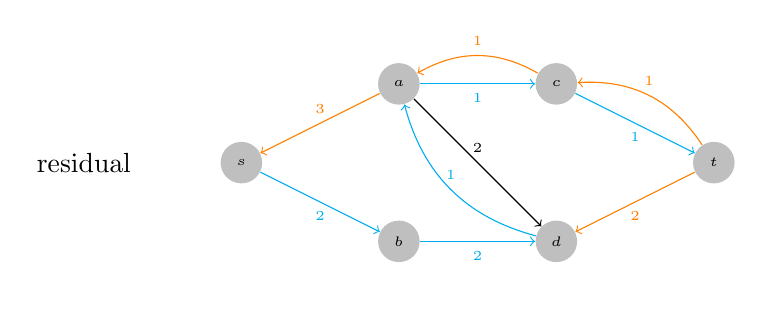
\begin{tikzpicture}
\node[vertex] at (0, 0) (s) {\tiny $s$};
\node[vertex] at (2, 1) (a) {\tiny $a$};
\node[vertex] at (2, -1) (b) {\tiny $b$};
\node[vertex] at (4, 1) (c) {\tiny $c$};
\node[vertex] at (4, -1) (d) {\tiny $d$};
\node[vertex] at (6, 0) (t) {\tiny $t$};
\draw[<-, orange] (s) edge node[anchor = south] {\tiny $3$} (a);
\draw[->, cyan] (s) edge node[anchor = north] {\tiny $2$} (b);
\draw[->, cyan] (a) edge node[anchor = north] {\tiny $1$} (c);
\draw[<-, orange] (a) edge[bend left] node[anchor = south] {\tiny $1$} (c);
\draw[<-, cyan] (a) edge[bend right] node[anchor = south] {\tiny $1$} (d);
\draw[->] (a) edge node[anchor = south] {\tiny $2$} (d);
\draw[->, cyan] (b) edge node[anchor = north] {\tiny $2$} (d);
\draw[<-, orange] (c) edge[bend left] node[anchor = south] {\tiny $1$} (t);
\draw[->, cyan] (c) edge node[anchor = north] {\tiny $1$} (t);
\draw[<-, orange] (d) edge node[anchor = north] {\tiny $2$} (t);
\draw[<-, white] (s) edge[bend right] node[anchor = north] {\tiny $1$} (b);
\draw[<-, white] (b) edge[bend right] node[anchor = north] {\tiny $1$} (d);

\node at (-2, 0) {residual};
\end{tikzpicture}
\end{center}
\end{frame}

\begin{frame} 
\begin{center}
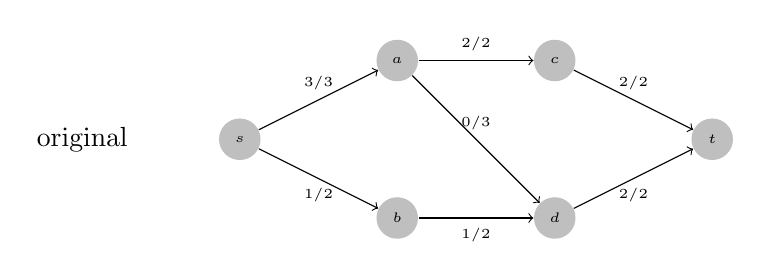
\begin{tikzpicture}
\node[vertex] at (0, 0) (s) {\tiny $s$};
\node[vertex] at (2, 1) (a) {\tiny $a$};
\node[vertex] at (2, -1) (b) {\tiny $b$};
\node[vertex] at (4, 1) (c) {\tiny $c$};
\node[vertex] at (4, -1) (d) {\tiny $d$};
\node[vertex] at (6, 0) (t) {\tiny $t$};
\draw[->] (s) edge node[anchor = south] {\tiny $3 / 3$} (a);
\draw[->] (s) edge node[anchor = north] {\tiny $1 / 2$} (b);
\draw[->] (a) edge node[anchor = south] {\tiny $2 / 2$} (c);
\draw[->] (a) edge node[anchor = south] {\tiny $0 / 3$} (d);
\draw[->] (b) edge node[anchor = north] {\tiny $1 / 2$} (d);
\draw[->] (c) edge node[anchor = south] {\tiny $2 / 2$} (t);
\draw[->] (d) edge node[anchor = north] {\tiny $2 / 2$} (t);
\node at (-2, 0) {original};
\end{tikzpicture}
\end{center}

\begin{center}
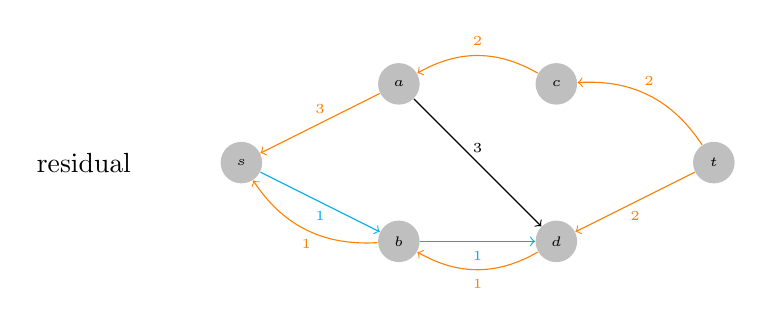
\begin{tikzpicture}
\node[vertex] at (0, 0) (s) {\tiny $s$};
\node[vertex] at (2, 1) (a) {\tiny $a$};
\node[vertex] at (2, -1) (b) {\tiny $b$};
\node[vertex] at (4, 1) (c) {\tiny $c$};
\node[vertex] at (4, -1) (d) {\tiny $d$};
\node[vertex] at (6, 0) (t) {\tiny $t$};
\draw[<-, orange] (s) edge node[anchor = south] {\tiny $3$} (a);
\draw[->, cyan] (s) edge node[anchor = north] {\tiny $1$} (b);
\draw[<-, orange] (s) edge[bend right] node[anchor = north] {\tiny $1$} (b);
\draw[<-, orange] (b) edge[bend right] node[anchor = north] {\tiny $1$} (d);

%\draw[->, cyan] (a) edge node[anchor = north] {\tiny $1$} (c);
\draw[<-, orange] (a) edge[bend left] node[anchor = south] {\tiny $2$} (c);
%\draw[<-, cyan] (a) edge[bend right] node[anchor = south] {\tiny $1$} (d);
\draw[->] (a) edge node[anchor = south] {\tiny $3$} (d);
\draw[->, cyan] (b) edge node[anchor = north] {\tiny $1$} (d);
\draw[<-, orange] (c) edge[bend left] node[anchor = south] {\tiny $2$} (t);
%\draw[->, cyan] (c) edge node[anchor = north] {\tiny $1$} (t);
\draw[<-, orange] (d) edge node[anchor = north] {\tiny $2$} (t);
\node at (-2, 0) {residual};
\end{tikzpicture}
\end{center}
\end{frame}


\begin{frame}[fragile]
\begin{itemize}
 \item The algorithm works directly on the residual graph $G_r$.
 
 \begin{enumerate}
  \item While there is an $s$-$t$ path $p$ in $G_r$
 \item \quad Push as much flow as possible through $p$
 \item \quad Update the residual graph $G_r$.
 \end{enumerate}

 \item One can show that this works.
 
 \item If we find paths with BFS we get an $O(|V| |E|^2)$ algorithm (aka. Edmonds-Karp algorithm).
 
 \item If we use DFS we get time complexity $O(|E| f^*)$ (aka. Ford-Fulkerson algorithm).
 
\end{itemize}

\end{frame}

% \begin{frame}[fragile]
%  \begin{lstlisting}
% int maxFlow(HashMap<Integer, Integer>[] g, int s, int t) {
%   // output 0 for s = t (convention)
%   if(s == t) return 0;
%   // initialize maxflow
%   int maxFlow = 0;
%   // compute an augmenting path
%   LinkedList<Edge> path = findAugmentingPath(g, s, t);
%   // loop while augmenting paths exists and update g
%   while(path != null) {
%     int pathCapacity = applyPath(g, path);
%     maxFlow += pathCapacity;
%     path = findAugmentingPath(g, s, t);
%   }
%   return maxFlow;
% }  
%  \end{lstlisting}
% \end{frame}
%  
%  \begin{frame}[fragile]
%  \begin{lstlisting}
% LinkedList<Edge> findAugmentingPath(HashMap<Integer,Integer>[] g, int s, int t){
%   // initialize the queue for BFS
%   Queue<Integer> Q = new LinkedList<Integer>();
%   Q.add(s);
%   // initialize the parent array for path reconstruction
%   Edge[] parent = new Edge[g.length];
%   Arrays.fill(parent, null);
%   // perform a BFS
%   while(!Q.isEmpty()) {
%     int cur = Q.poll();
%     for(Entry<Integer, Integer> e : g[cur].entrySet()) {
%       int next = e.getKey();
%       int w = e.getValue();
%       if(parent[next] == null) {
%         Q.add(next);
%         parent[next] = new Edge(cur, next, w);
%       }
%     }
%   }
%   // reconstruct the path
%   if(parent[t] == null) return null;
%   LinkedList<Edge> path = new LinkedList<Edge>();
%   int cur = t;
%   while(cur != s) {
%     path.add(parent[cur]);
%     cur = parent[cur].orig;
%   }
%   return path;
% }
% \end{lstlisting}
% \end{frame}
%  
%  \begin{frame}[fragile]
%  \begin{lstlisting}
% int applyPath(HashMap<Integer, Integer>[] g, LinkedList<Edge> path) {
%   int minCapacity = Integer.MAX_VALUE;
%   for(Edge e : path) {
%     minCapacity = Math.min(minCapacity, e.w);
%   }
%   for(Edge e : path) {
%     // treat path edge
%     if(minCapacity == e.w) {
%       // the capacity became 0, remove edge
%       g[e.orig].remove(e.dest);
%     } else {
%       // there remains capacity, update capacity
%       g[e.orig].put(e.dest, e.w - minCapacity);
%     }
%     // treat back edge
%     Integer backCapacity = g[e.dest].get(e.orig);
%     if(backCapacity == null) { 
%       // the back edge does not exist yet
%       g[e.dest].put(e.orig, minCapacity);
%     } else {
%       // the back edge already exists, update capacity
%       g[e.dest].put(e.orig, backCapacity + minCapacity);
%     }
%   }
%   return minCapacity;
% }
%  \end{lstlisting}
% 
% \end{frame}

\begin{frame}
\begin{center}
{\color{black} \huge{\textbf{Minimum cut}}}
\end{center}
\end{frame}

\begin{frame}

The \textbf{Minimum-cut} problem consits of finding a set of edges whose removal
disconnects two nodes in the network and has minimal cost. The cost of removing an edge
is given by its weight.

\vspace{2cm}

\pause

Ideas?...

\end{frame}


\begin{frame}
\begin{center}
\includegraphics[scale = 0.8]{mincut.jpg}
\end{center}
\end{frame}


%\begin{frame}
%\begin{center}
%\includegraphics[scale = 0.5]{wow.png}
%\end{center}
%\end{frame}

\begin{frame}
\begin{center}
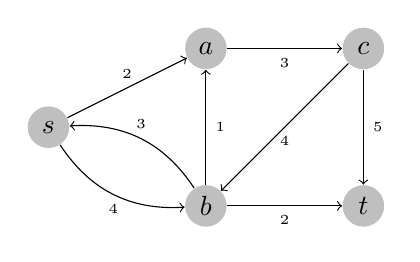
\begin{tikzpicture}
\node[vertex] at (0, 0) (s) {$s$};
\node[vertex] at (2, 1) (a) {$a$};
\node[vertex] at (2, -1) (b) {$b$};
\node[vertex] at (4, 1) (c) {$c$};
\node[vertex] at (4, -1) (t) {$t$};
\draw[->] (s) edge node[anchor = south] {\tiny $2$} (a);
\draw[->] (s) edge[bend right] node[anchor = north] {\tiny $4$} (b);
\draw[->] (a) edge node[anchor = north] {\tiny $3$} (c);
\draw[->] (b) edge[bend right] node[anchor = south] {\tiny $3$} (s);
\draw[->] (b) edge node[anchor = west] {\tiny $1$} (a);
\draw[->] (c) edge node[anchor = north] {\tiny $4$} (b);
\draw[->] (b) edge node[anchor = north] {\tiny $2$} (t);
\draw[->] (c) edge node[anchor = west] {\tiny $5$} (t);
%\draw[->] (a) edge node{$2$} (t);
\end{tikzpicture}
\end{center}

\end{frame}

\begin{frame}
Max-flow:
\begin{center}
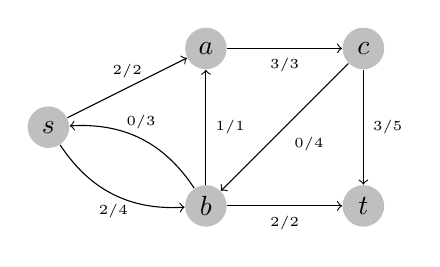
\begin{tikzpicture}
\node[vertex] at (0, 0) (s) {$s$};
\node[vertex] at (2, 1) (a) {$a$};
\node[vertex] at (2, -1) (b) {$b$};
\node[vertex] at (4, 1) (c) {$c$};
\node[vertex] at (4, -1) (t) {$t$};
\draw[->] (s) edge node[anchor = south] {\tiny $2/2$} (a);
\draw[->] (s) edge[bend right] node[anchor = north] {\tiny $2/4$} (b);
\draw[->] (a) edge node[anchor = north] {\tiny $3/3$} (c);
\draw[->] (b) edge[bend right] node[anchor = south] {\tiny $0/3$} (s);
\draw[->] (b) edge node[anchor = west] {\tiny $1/1$} (a);
\draw[->] (c) edge node[anchor = north west] {\tiny $0/4$} (b);
\draw[->] (b) edge node[anchor = north] {\tiny $2/2$} (t);
\draw[->] (c) edge node[anchor = west] {\tiny $3/5$} (t);
%\draw[->] (a) edge node{$2$} (t);
\end{tikzpicture}
\end{center}

\end{frame}

\begin{frame}
Look at the nodes reachable from $s$ in the residual graph.
\begin{center}
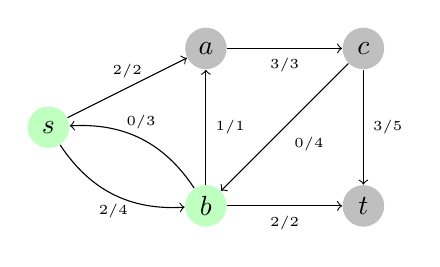
\begin{tikzpicture}
\node[visited] at (0, 0) (s) {$s$};
\node[vertex] at (2, 1) (a) {$a$};
\node[visited] at (2, -1) (b) {$b$};
\node[vertex] at (4, 1) (c) {$c$};
\node[vertex] at (4, -1) (t) {$t$};
\draw[->] (s) edge node[anchor = south] {\tiny $2/2$} (a);
\draw[->] (s) edge[bend right] node[anchor = north] {\tiny $2/4$} (b);
\draw[->] (a) edge node[anchor = north] {\tiny $3/3$} (c);
\draw[->] (b) edge[bend right] node[anchor = south] {\tiny $0/3$} (s);
\draw[->] (b) edge node[anchor = west] {\tiny $1/1$} (a);
\draw[->] (c) edge node[anchor = north west] {\tiny $0/4$} (b);
\draw[->] (b) edge node[anchor = north] {\tiny $2/2$} (t);
\draw[->] (c) edge node[anchor = west] {\tiny $3/5$} (t);
\end{tikzpicture}
\end{center}

\end{frame}


\begin{frame}
The minimum cut consists of the edges between the two sets.
\begin{center}
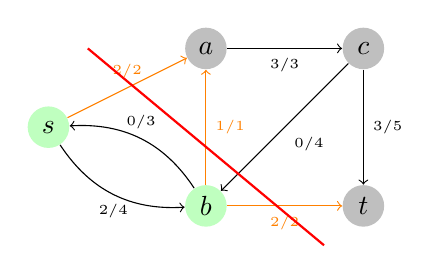
\begin{tikzpicture}
\node[visited] at (0, 0) (s) {$s$};
\node[vertex] at (2, 1) (a) {$a$};
\node[visited] at (2, -1) (b) {$b$};
\node[vertex] at (4, 1) (c) {$c$};
\node[vertex] at (4, -1) (t) {$t$};
\draw[->, orange] (s) edge node[anchor = south] {\tiny $2/2$} (a);
\draw[->] (s) edge[bend right] node[anchor = north] {\tiny $2/4$} (b);
\draw[->] (a) edge node[anchor = north] {\tiny $3/3$} (c);
\draw[->] (b) edge[bend right] node[anchor = south] {\tiny $0/3$} (s);
\draw[->, orange] (b) edge node[anchor = west] {\tiny $1/1$} (a);
\draw[->] (c) edge node[anchor = north west] {\tiny $0/4$} (b);
\draw[->, orange] (b) edge node[anchor = north] {\tiny $2/2$} (t);
\draw[->] (c) edge node[anchor = west] {\tiny $3/5$} (t);
\draw[thick, red] (0.5, 1) -- (3.5, -1.5);
\end{tikzpicture}
\end{center}
\pause
Also known as the \textbf{Min-Cut Max-Flow theorem}:
$$
\textsf{Max-Flow}(s, t, G) = \textsf{Min-Cut}(s, t, G)
$$
\end{frame}


\begin{frame}
\begin{center}
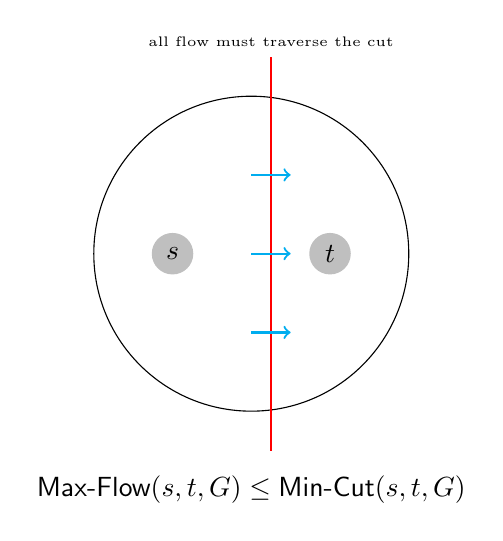
\begin{tikzpicture}
\draw (0, 0) circle (2);
\node[vertex] at (-1, 0) {$s$};
\node[vertex] at (1, 0) {$t$};

\pause

\draw[thick, red] (0.25, -2.5) -- (0.25, 2.5) node[black, anchor = south] {\tiny all flow must traverse the cut};
\draw[->, thick, cyan] (0, 0) -- (0.5, 0);
\draw[->, thick, cyan] (0, -1) -- (0.5, -1);
\draw[->, thick, cyan] (0, 1) -- (0.5, 1);

\pause

\node at (0, -3) {$\textsf{Max-Flow}(s, t, G) \leq \textsf{Min-Cut}(s, t, G)$};

\end{tikzpicture}
\end{center}
\end{frame}

\begin{frame}

Suppose that $\textsf{Max-Flow}(s, t, G) < \textsf{Min-Cut}(s, t, G)$

\begin{center}
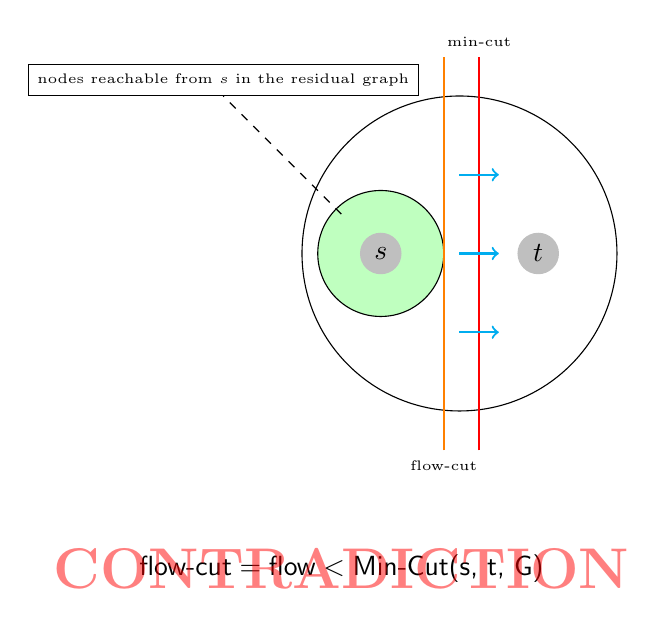
\begin{tikzpicture}
\draw (0, 0) circle (2);
\node[vertex] at (-1, 0) {$s$};
\node[vertex] at (1, 0) {$t$};

\draw[thick, red] (0.25, -2.5) -- (0.25, 2.5) node[black, anchor = south] {\tiny min-cut};
\draw[->, thick, cyan] (0, 0) -- (0.5, 0);
\draw[->, thick, cyan] (0, -1) -- (0.5, -1);
\draw[->, thick, cyan] (0, 1) -- (0.5, 1);

\pause 

\draw[fill = green!25!white] (-1, 0) circle (0.8);

\draw[dashed] (-1.5, 0.5) -- (-3, 2) node[draw, solid, anchor = south] {\tiny nodes reachable from $s$ in the residual graph};

\node[vertex] at (-1, 0) {$s$};

\pause

\draw[thick, orange] (-0.2, -2.5) node[black, anchor = north] {\tiny flow-cut} -- (-0.2, 2.5);

\pause

\node at (-1.5, -4) {$\textsf{flow-cut} = \textsf{flow} < \textsf{Min-Cut(s, t, G)}$};

\pause

\node[red, opacity = 0.5] at (-1.5, -4) {\huge \textbf{CONTRADICTION}};


\end{tikzpicture}
\end{center}
\end{frame}

\begin{frame}
\begin{center}
{\color{black} \huge{\textbf{Related problems and modeling}}}
\end{center}
\end{frame}

\begin{frame}
\textbf{Node capacities:}

\begin{center}
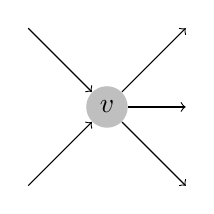
\begin{tikzpicture}
\node[vertex] (v) at (0, 0) {$v$};
\draw[->] (-1, 1) -- (v);
\draw[->] (-1, -1) -- (v);
\draw[->] (v) -- (1, 0);
\draw[->] (v) -- (1, 1);
\draw[->] (v) -- (1, -1);
\end{tikzpicture} 
\end{center}

Split nodes:

\begin{center}
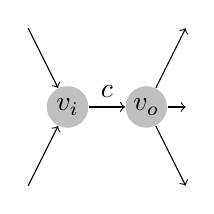
\begin{tikzpicture}
\node[vertex] (vi) at (-0.5, 0) {$v_{i}$};
\node[vertex] (vo) at (0.5, 0) {$v_{o}$};
\draw[->] (-1, 1) -- (vi);
\draw[->] (-1, -1) -- (vi);
\draw[->] (vo) -- (1, 0);
\draw[->] (vo) -- (1, 1);
\draw[->] (vo) -- (1, -1);
\draw[->] (vi) edge node[anchor = south] {$c$} (vo);
\end{tikzpicture} 
\end{center}
 
\end{frame}

\begin{frame}
\textbf{Multiple sources / sinks:}

\begin{center}
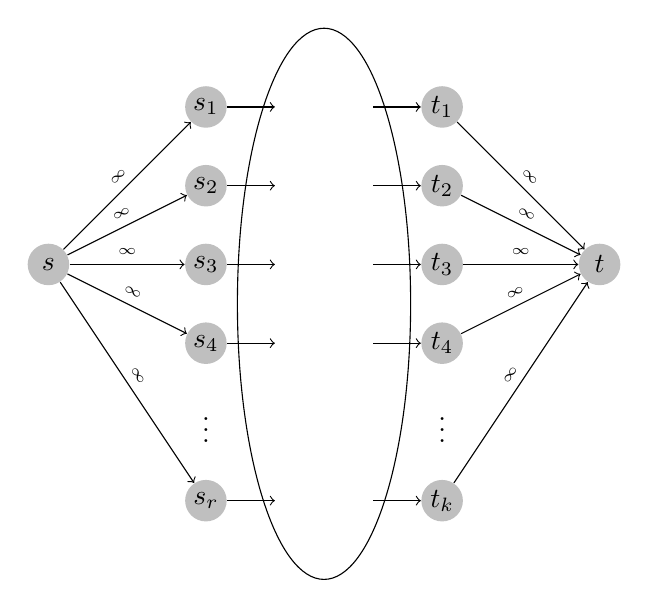
\begin{tikzpicture}
\node[vertex] (s) at (-2, 0) {$s$};

\node[vertex] (s1) at (0, 2) {$s_1$};
\node[vertex] (s2) at (0, 1) {$s_2$};
\node[vertex] (s3) at (0, 0) {$s_3$};
\node[vertex] (s4) at (0, -1) {$s_4$};
\node (d1) at (0, -2) {$\vdots$};
\node[vertex] (s5) at (0, -3) {$s_r$};


\node (ss1) at (1, 2) {};
\node (ss2) at (1, 1) {};
\node (ss3) at (1, 0) {};
\node (ss4) at (1, -1) {};
\node (ss5) at (1, -3) {};

\node (tt1) at (2, 2) {};
\node (tt2) at (2, 1) {};
\node (tt3) at (2, 0) {};
\node (tt4) at (2, -1) {};
\node (tt5) at (2, -3) {};


\node[vertex] (t1) at (3, 2) {$t_1$};
\node[vertex] (t2) at (3, 1) {$t_2$};
\node[vertex] (t3) at (3, 0) {$t_3$};
\node[vertex] (t4) at (3, -1) {$t_4$};
\node (d2) at (3, -2) {$\vdots$};
\node[vertex] (t5) at (3, -3) {$t_k$};

\node[vertex] (t) at (5, 0) {$t$};

\draw[->] (s) edge[midway, pos=0.5, sloped, above] node {\tiny $\infty$} (s1);
\draw[->] (s) edge[midway, pos=0.5, sloped, above] node {\tiny $\infty$} (s2);
\draw[->] (s) edge[midway, pos=0.5, sloped, above] node {\tiny $\infty$} (s3);
\draw[->] (s) edge[midway, pos=0.5, sloped, above] node {\tiny $\infty$} (s4);
\draw[->] (s) edge[midway, pos=0.5, sloped, above] node {\tiny $\infty$} (s5);

\draw[->] (t1) edge[midway, pos=0.5, sloped, above] node {\tiny $\infty$} (t);
\draw[->] (t2) edge[midway, pos=0.5, sloped, above] node {\tiny $\infty$} (t);
\draw[->] (t3) edge[midway, pos=0.5, sloped, above] node {\tiny $\infty$} (t);
\draw[->] (t4) edge[midway, pos=0.5, sloped, above] node {\tiny $\infty$} (t);
\draw[->] (t5) edge[midway, pos=0.5, sloped, above] node {\tiny $\infty$} (t);

\draw[->] (s1) -- (ss1);
\draw[->] (s2) -- (ss2);
\draw[->] (s3) -- (ss3);
\draw[->] (s4) -- (ss4);
\draw[->] (s5) -- (ss5);

\draw[->] (tt1) -- (t1);
\draw[->] (tt2) -- (t2);
\draw[->] (tt3) -- (t3);
\draw[->] (tt4) -- (t4);
\draw[->] (tt5) -- (t5);

\draw (1.5, -0.5) ellipse (1.1cm and 3.5cm);

\end{tikzpicture} 
\end{center}

\end{frame}

\begin{frame}
\textbf{Maximum bipartite matching:}

\vspace{1cm}

There are $N$ women and $M$ men. Each woman is interested in some of the men.
The goal is to find maximum number of couples that can be formed.

\end{frame}

\begin{frame}
\begin{center}
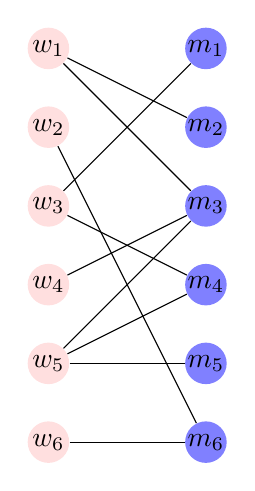
\begin{tikzpicture}
\node[woman] (w1) at (0, 5) {$w_1$};
\node[woman] (w2) at (0, 4) {$w_2$};
\node[woman] (w3) at (0, 3) {$w_3$};
\node[woman] (w4) at (0, 2) {$w_4$};
\node[woman] (w5) at (0, 1) {$w_5$};
\node[woman] (w6) at (0, 0) {$w_6$};


\node[men] (m1) at (2, 5) {$m_1$};
\node[men] (m2) at (2, 4) {$m_2$};
\node[men] (m3) at (2, 3) {$m_3$};
\node[men] (m4) at (2, 2) {$m_4$};
\node[men] (m5) at (2, 1) {$m_5$};
\node[men] (m6) at (2, 0) {$m_6$};

\draw (w1) -- (m2);
\draw (w1) -- (m3);
\draw (w3) -- (m1);
\draw (w3) -- (m4);
\draw (w4) -- (m3);
\draw (w5) -- (m3);
\draw (w5) -- (m4);
\draw (w6) -- (m6);
\draw (w2) -- (m6);
\draw (w5) -- (m5);

\end{tikzpicture}
\end{center}
\end{frame}

\begin{frame}
\begin{center}
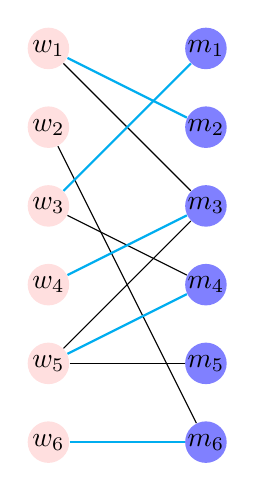
\begin{tikzpicture}
\node[woman] (w1) at (0, 5) {$w_1$};
\node[woman] (w2) at (0, 4) {$w_2$};
\node[woman] (w3) at (0, 3) {$w_3$};
\node[woman] (w4) at (0, 2) {$w_4$};
\node[woman] (w5) at (0, 1) {$w_5$};
\node[woman] (w6) at (0, 0) {$w_6$};


\node[men] (m1) at (2, 5) {$m_1$};
\node[men] (m2) at (2, 4) {$m_2$};
\node[men] (m3) at (2, 3) {$m_3$};
\node[men] (m4) at (2, 2) {$m_4$};
\node[men] (m5) at (2, 1) {$m_5$};
\node[men] (m6) at (2, 0) {$m_6$};

\draw (w1) -- (m3);
\draw (w3) -- (m4);
\draw (w5) -- (m3);
\draw (w2) -- (m6);
\draw (w5) -- (m5);
\draw[thick, cyan] (w5) -- (m4);
\draw[thick, cyan] (w6) -- (m6);
\draw[thick, cyan] (w4) -- (m3);
\draw[thick, cyan] (w3) -- (m1);
\draw[thick, cyan] (w1) -- (m2);

\end{tikzpicture}
\end{center}
\end{frame}


\begin{frame}
\begin{center}
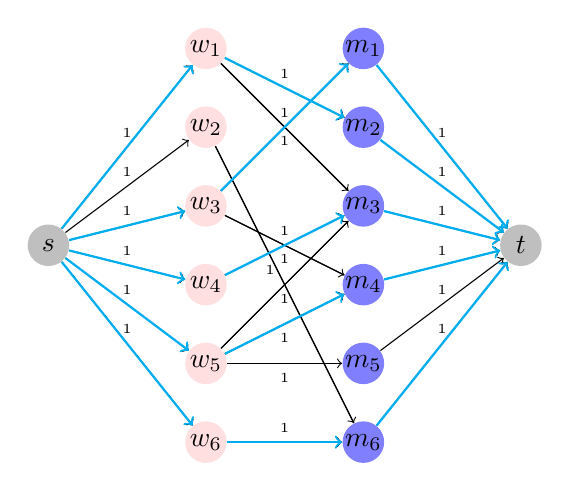
\begin{tikzpicture}
\node[woman] (w1) at (0, 5) {$w_1$};
\node[woman] (w2) at (0, 4) {$w_2$};
\node[woman] (w3) at (0, 3) {$w_3$};
\node[woman] (w4) at (0, 2) {$w_4$};
\node[woman] (w5) at (0, 1) {$w_5$};
\node[woman] (w6) at (0, 0) {$w_6$};


\node[men] (m1) at (2, 5) {$m_1$};
\node[men] (m2) at (2, 4) {$m_2$};
\node[men] (m3) at (2, 3) {$m_3$};
\node[men] (m4) at (2, 2) {$m_4$};
\node[men] (m5) at (2, 1) {$m_5$};
\node[men] (m6) at (2, 0) {$m_6$};

\draw (w1) -- (m3);
\draw (w3) -- (m4);
\draw (w5) -- (m3);
\draw (w2) -- (m6);
\draw (w5) -- (m5);
\draw (w5) -- (m4);
\draw (w6) -- (m6);
\draw (w4) -- (m3);
\draw (w3) -- (m1);
\draw (w1) -- (m2);

\node[vertex] (s) at (-2, 2.5) {$s$};
\node[vertex] (t) at (4, 2.5) {$t$};

\pause

\draw[->] (s) edge node[anchor = south] {\tiny 1} (w1);
\draw[->] (s) edge node[anchor = south] {\tiny 1} (w2);
\draw[->] (s) edge node[anchor = south] {\tiny 1} (w3);
\draw[->] (s) edge node[anchor = south] {\tiny 1} (w4);
\draw[->] (s) edge node[anchor = south] {\tiny 1} (w5);
\draw[->] (s) edge node[anchor = south] {\tiny 1} (w6);

\draw[->] (m1) edge node[anchor = south] {\tiny 1} (t);
\draw[->] (m2) edge node[anchor = south] {\tiny 1} (t);
\draw[->] (m3) edge node[anchor = south] {\tiny 1} (t);
\draw[->] (m4) edge node[anchor = south] {\tiny 1} (t);
\draw[->] (m5) edge node[anchor = south] {\tiny 1} (t);
\draw[->] (m6) edge node[anchor = south] {\tiny 1} (t);

\pause


\draw[->] (w1) edge node[anchor = south] {\tiny 1} (m2);
\draw[->] (w1) edge node[anchor = south] {\tiny 1} (m3);
\draw[->] (w3) edge node[anchor = north] {\tiny 1} (m1);
\draw[->] (w3) edge node[anchor = south] {\tiny 1} (m4);
\draw[->] (w4) edge node[anchor = north] {\tiny 1} (m3);
\draw[->] (w5) edge node[anchor = north] {\tiny 1} (m3);
\draw[->] (w5) edge node[anchor = north] {\tiny 1} (m4);
\draw[->] (w6) edge node[anchor = south] {\tiny 1} (m6);
\draw[->] (w2) edge node[anchor = south east] {\tiny 1} (m6);
\draw[->] (w5) edge node[anchor = north] {\tiny 1} (m5);

\pause 

\draw[->, thick, cyan] (s) -- (w1);
\draw[->, thick, cyan] (s) -- (w3);
\draw[->, thick, cyan] (s) -- (w4);
\draw[->, thick, cyan] (s) -- (w5);
\draw[->, thick, cyan] (s) -- (w6);

\draw[->, thick, cyan] (m1) -- (t);
\draw[->, thick, cyan] (m2) -- (t);
\draw[->, thick, cyan] (m3) -- (t);
\draw[->, thick, cyan] (m4) -- (t);
\draw[->, thick, cyan] (m6) -- (t);


\draw[->, thick, cyan] (w5) -- (m4);
\draw[->, thick, cyan] (w6) -- (m6);
\draw[->, thick, cyan] (w4) -- (m3);
\draw[->, thick, cyan] (w3) -- (m1);
\draw[->, thick, cyan] (w1) -- (m2);

\end{tikzpicture}
\end{center}
\end{frame}


\begin{frame}
\begin{center}
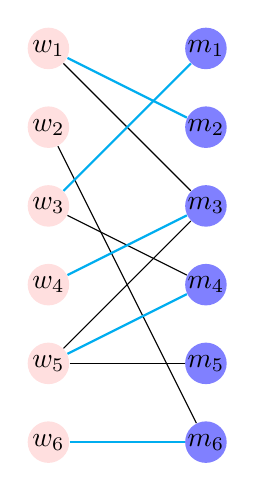
\begin{tikzpicture}
\node[woman] (w1) at (0, 5) {$w_1$};
\node[woman] (w2) at (0, 4) {$w_2$};
\node[woman] (w3) at (0, 3) {$w_3$};
\node[woman] (w4) at (0, 2) {$w_4$};
\node[woman] (w5) at (0, 1) {$w_5$};
\node[woman] (w6) at (0, 0) {$w_6$};


\node[men] (m1) at (2, 5) {$m_1$};
\node[men] (m2) at (2, 4) {$m_2$};
\node[men] (m3) at (2, 3) {$m_3$};
\node[men] (m4) at (2, 2) {$m_4$};
\node[men] (m5) at (2, 1) {$m_5$};
\node[men] (m6) at (2, 0) {$m_6$};

\draw (w1) -- (m3);
\draw (w3) -- (m4);
\draw (w5) -- (m3);
\draw (w2) -- (m6);
\draw (w5) -- (m5);
\draw[thick, cyan] (w5) -- (m4);
\draw[thick, cyan] (w6) -- (m6);
\draw[thick, cyan] (w4) -- (m3);
\draw[thick, cyan] (w3) -- (m1);
\draw[thick, cyan] (w1) -- (m2);

\end{tikzpicture}
\end{center}
\end{frame}

\begin{frame}
\textbf{Min Path Cover on DAG:}

\vspace{1cm}

Given a DAG compute the minimum number of \textbf{node disjoint} paths required to cover all the nodes.

\end{frame}


\begin{frame}

\begin{center}
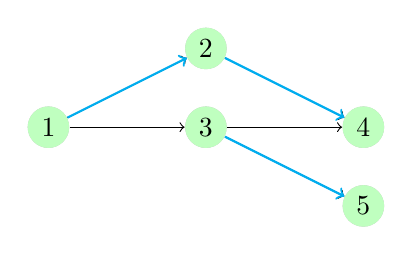
\begin{tikzpicture}
\node[vertex] (1) at (0, 0) {1};
\node[vertex] (2) at (2, 1) {2};
\node[vertex] (3) at (2, 0) {3};
\node[vertex] (4) at (4, 0) {4};
\node[vertex] (5) at (4, -1) {5};
\draw[->] (1) -- (3);
\draw[->] (3) -- (4);
\draw[->] (1) -- (2);
\draw[->] (2) -- (4);
\draw[->] (3) -- (5);

\pause

\draw[->, thick, cyan] (1) -- (2);
\draw[->, thick, cyan] (2) -- (4);

\node[visited] (1) at (0, 0) {1};
\node[visited] (2) at (2, 1) {2};
\node[visited] (4) at (4, 0) {4};

\pause

\draw[->, thick, cyan] (3) -- (5);

\node[visited] (3) at (2, 0) {3};
\node[visited] (5) at (4, -1) {5};

\end{tikzpicture}
\end{center}
\end{frame}

\begin{frame}[fragile]
Define a bipartite graph containing the edges of input graph:

\begin{center}
\begin{tabular}{ccc}  
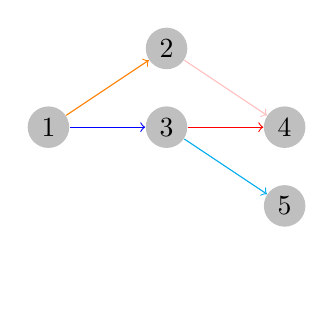
\begin{tikzpicture}
\node[vertex] (1) at (0, 0) {1};
\node[vertex] (2) at (1.5, 1) {2};
\node[vertex] (3) at (1.5, 0) {3};
\node[vertex] (4) at (3, 0) {4};
\node[vertex] (5) at (3, -1) {5};
\draw[blue, ->] (1) -- (3);
\draw[red, ->] (3) -- (4);
\draw[orange, ->] (1) -- (2);
\draw[pink, ->] (2) -- (4);
\draw[cyan, ->] (3) -- (5);
\node at (0, -2) {};
\end{tikzpicture}

&
\hspace{1cm} 
& 
 
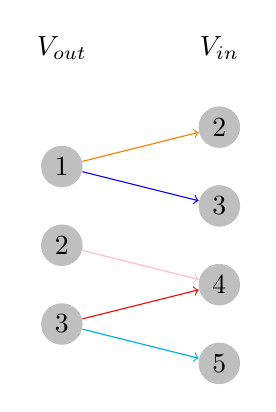
\begin{tikzpicture}
\node[vertex] (1)  at (0, 0)    {1};
\node[vertex] (2)  at (0, -1)   {2};
\node[vertex] (3)  at (0, -2)   {3};
\node[vertex] (22) at (2, 0.5)  {2};
\node[vertex] (33) at (2, -0.5) {3};
\node[vertex] (44) at (2, -1.5) {4};
\node[vertex] (55) at (2, -2.5) {5};

\draw[->, orange] (1) -- (22);
\draw[->, pink] (2) -- (44);
\draw[->, blue] (1) -- (33);
\draw[->, red] (3) -- (44);
\draw[->, cyan] (3) -- (55);

\node at (0, 1.5) {$V_{out}$};
\node at (2, 1.5) {$V_{in}$};

\end{tikzpicture}
\end{tabular}
\end{center}

\end{frame}


\begin{frame}[fragile]
Compute maximum bipartite matching.

\begin{center}
\begin{tabular}{ccc}  
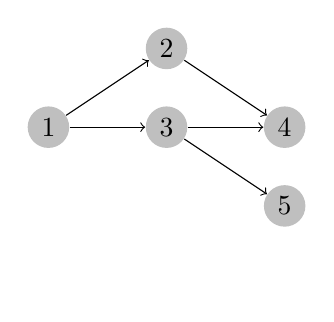
\begin{tikzpicture}
\node[vertex] (1) at (0, 0) {1};
\node[vertex] (2) at (1.5, 1) {2};
\node[vertex] (3) at (1.5, 0) {3};
\node[vertex] (4) at (3, 0) {4};
\node[vertex] (5) at (3, -1) {5};
\draw[->] (1) -- (3);
\draw[->] (3) -- (4);
\draw[->] (1) -- (2);
\draw[->] (2) -- (4);
\draw[->] (3) -- (5);
\node at (0, -2) {};
\end{tikzpicture}

&
\hspace{1cm} 
& 
 
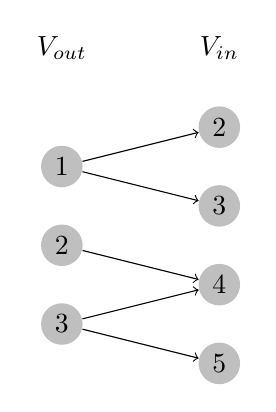
\begin{tikzpicture}
\node[vertex] (1)  at (0, 0)    {1};
\node[vertex] (2)  at (0, -1)   {2};
\node[vertex] (3)  at (0, -2)   {3};
\node[vertex] (22) at (2, 0.5)  {2};
\node[vertex] (33) at (2, -0.5) {3};
\node[vertex] (44) at (2, -1.5) {4};
\node[vertex] (55) at (2, -2.5) {5};

\draw[->] (1) -- (22);
\draw[->] (2) -- (44);
\draw[->] (1) -- (33);
\draw[->] (3) -- (44);
\draw[->] (3) -- (55);

\node at (0, 1.5) {$V_{out}$};
\node at (2, 1.5) {$V_{in}$};

\end{tikzpicture}
\end{tabular}
\end{center}

\end{frame}



\begin{frame}[fragile]
Compute maximum bipartite matching.

\begin{center}
\begin{tabular}{ccc}  
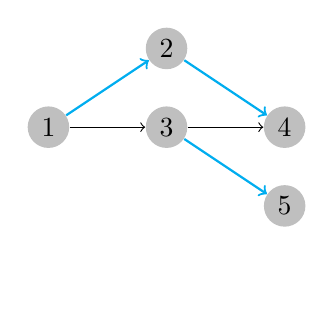
\begin{tikzpicture}
\node[vertex] (1) at (0, 0) {1};
\node[vertex] (2) at (1.5, 1) {2};
\node[vertex] (3) at (1.5, 0) {3};
\node[vertex] (4) at (3, 0) {4};
\node[vertex] (5) at (3, -1) {5};
\draw[->] (1) -- (3);
\draw[->] (3) -- (4);
\draw[->, thick, cyan] (1) -- (2);
\draw[->, thick, cyan] (2) -- (4);
\draw[->, thick, cyan] (3) -- (5);
\node at (0, -2) {};
\end{tikzpicture}

&
\hspace{1cm} 
& 
 
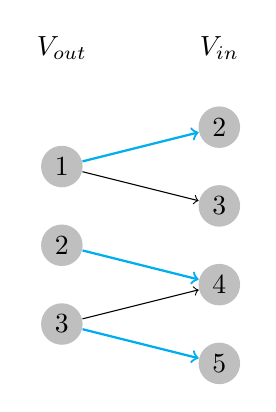
\begin{tikzpicture}
\node[vertex] (1)  at (0, 0)    {1};
\node[vertex] (2)  at (0, -1)   {2};
\node[vertex] (3)  at (0, -2)   {3};
\node[vertex] (22) at (2, 0.5)  {2};
\node[vertex] (33) at (2, -0.5) {3};
\node[vertex] (44) at (2, -1.5) {4};
\node[vertex] (55) at (2, -2.5) {5};

\draw[->, thick, cyan] (1) -- (22);
\draw[->, thick, cyan] (2) -- (44);
\draw[->] (1) -- (33);
\draw[->] (3) -- (44);
\draw[->, thick, cyan] (3) -- (55);

\node at (0, 1.5) {$V_{out}$};
\node at (2, 1.5) {$V_{in}$};

\end{tikzpicture}
\end{tabular}
\end{center}

\pause 


\begin{tikzpicture}[overlay]
\node at (2, 0) {\includegraphics[scale = 0.2]{paths.jpg}};
\end{tikzpicture}

\end{frame}

\begin{frame}
 
\begin{itemize}
 \item The $n$ nodes can be covered with $n$ paths of length $0$.
 \vspace{0.5cm}
 \item Matching nodes $a$ and $b$ says that we can use one less path.
 \vspace{0.5cm}
 \item If the MCBM has size $m$, then we just need $n - m$ paths. 
\end{itemize}
 
\pause 
 
\vspace{0.5cm} 
 
\textbf{Variants:}

\begin{enumerate}
 
 \item What if we do not require node disjoint paths?
 
 \pause
 
 \vspace{0.25cm}
 
 Same algorithm but on the \textbf{transitive closure}.

 \pause
 
 \vspace{0.5cm}
 
 \item Edge disjoint paths.
 
 \pause
 $$
 \sum_{v \in V} \max \left( \delta^+(v) - \delta^-(v), 0 \right)
 $$
 
\end{enumerate}

 
\end{frame}

\begin{frame}

\textbf{Maximum edje-disjoint paths:}

\vspace{1cm}

Given a graph and two nodes $s$ and $t$ compute the maximum number edge disjoint paths
between them.
 
\pause

\vspace{0.5cm}

\textbf{Solution:}

Set a unit capacity on every edge and compute the maximum flow.

\vspace{0.5cm}

\textbf{What about node-disjoint paths?}

\pause

Set also a unit capacity on every node (by slitting).

\end{frame}

\begin{frame}
\begin{center}
{\color{black} \huge{\textbf{Minimum cost maximum flow}}}
\end{center}
\end{frame}

\begin{frame}

\textbf{Minimum cost flow:}

\vspace{0.5cm}

Same problem as max-flow but each edge has a weight on the edges. Find the cheapest possible
way of sending some information through the network. The weight represents the cost \textbf{per unit of flow}.

\pause

\begin{center}
\includegraphics[scale = 0.5]{hard.jpg}
\end{center}

\end{frame}


\begin{frame}[fragile]
\textbf{Residual graph} for minimum cost flow:

\vspace{1cm}

Original

\begin{center}
\begin{tikzpicture}
\node[vertex] at (0, 0) (v) {\tiny $v$};
\node[vertex] at (2, 0) (u) {\tiny $u$};
\draw[->] (v) edge node[anchor = south] {$f / c, w$} (u);
\end{tikzpicture}
\end{center}

\vspace{1cm}

Residual

\begin{center}
\begin{tikzpicture}
\node[vertex] at (0, 0) (v) {\tiny $v$};
\node[vertex] at (2, 0) (u) {\tiny $u$};
\draw[->] (v) edge[bend left] node[anchor = south] {$c - f, w$} (u);
\draw[<-, orange] (v) edge[bend right] node[anchor = north] {$f, -w$} (u);
\end{tikzpicture}
\end{center}

\end{frame}

\begin{frame}[fragile]

Same intuition as before: residual edges reverse choices.

\vspace{0.5cm}

Therefore we must undo what we payed $\Rightarrow \text{weight } = -w$.

\vspace{0.5cm}

\textbf{How to we find paths?} BFS? DFS? Dijkstra? Other?

\pause

\vspace{0.5cm}

Bellman-Ford! (negative edge costs)

\vspace{0.5cm}

\textbf{When do we stop?} 

\pause

\vspace{0.5cm}

No shortest path $\Leftrightarrow$ A negative cycle exists

\vspace{0.5cm}

\textbf{Complexity:} $O(m C U)$  with $C$ is max cap and $U$ is max cost.

\end{frame}

\begin{frame}[fragile]

There are many other (and faster) algorithms for the min-cost flow
problem. 

\vspace{0.5cm}

This problem is still rare in CP so we will only see this one.

\vspace{0.5cm}

It might be too slow for CP one day...

\end{frame}

\begin{frame}

\textbf{Maximum assignment problem:}

\vspace{0.5cm}

There are $N$ women and $N$ men. We have a compatibility matrix $P$ such that
$P[w][m]$ gives a score to the couple $(w, m)$. Make $N$ couples while
maximizing the sum of the compatibilities.

\end{frame}

\begin{frame}[fragile]

\begin{center}
\begin{tabular}{cccc}
  & $m_0$                       & $m_1$                       & $m_2$ \\
\cline{2-4}
$w_0$ & \multicolumn{1}{|c|}{1} & \multicolumn{1}{|c|}{3} & \multicolumn{1}{|c|}{2}  \\
\cline{2-4}
$w_1$ & \multicolumn{1}{|c|}{2} & \multicolumn{1}{|c|}{1} & \multicolumn{1}{|c|}{7}  \\
\cline{2-4}
$w_2$ & \multicolumn{1}{|c|}{5} & \multicolumn{1}{|c|}{4} & \multicolumn{1}{|c|}{9}  \\
\cline{2-4}
\end{tabular}
\end{center}

\vspace{0.5cm}

\begin{center}
\begin{tikzpicture}
\node[vertex] (w0) at (0, 1)  {$w_0$};
\node[vertex] (w1) at (0, 0) {$w_1$};
\node[vertex] (w2) at (0, -1) {$w_2$};

\node[vertex] (m0) at (2, 1)  {$m_0$};
\node[vertex] (m1) at (2, 0) {$m_1$};
\node[vertex] (m2) at (2, -1) {$m_2$};

\draw (w0) edge[pos=0.1, sloped] node[red] {\tiny $1$} (m0);
\draw (w0) edge[pos=0.25, sloped] node[red] {\tiny $3$} (m1);
\draw (w0) edge[pos=0.1, sloped] node[red] {\tiny $2$} (m2);

\draw (m0) edge[pos=0.1, sloped] node[red] {\tiny $2$} (w1);
\draw (m1) edge[pos=0.1, sloped] node[red] {\tiny $1$} (w1);
\draw (m2) edge[pos=0.2, sloped] node[red] {\tiny $7$} (w1);

\draw (w2) edge[pos=0.1, sloped] node[red] {\tiny $5$} (m0);
\draw (w2) edge[pos=0.25, sloped] node[red] {\tiny $4$} (m1);
\draw (w2) edge[pos=0.1, sloped] node[red] {\tiny $9$} (m2);

\end{tikzpicture}
\end{center}
\end{frame}

\begin{frame}[fragile]

\begin{center}
\begin{tabular}{cccc}
  & $m_0$                       & $m_1$                       & $m_2$ \\
\cline{2-4}
$w_0$ & \multicolumn{1}{|c|}{1} & \multicolumn{1}{|c|}{{\color{cyan} \textbf{3}}} & \multicolumn{1}{|c|}{2}  \\
\cline{2-4}
$w_1$ & \multicolumn{1}{|c|}{2} & \multicolumn{1}{|c|}{1} & \multicolumn{1}{|c|}{{\color{cyan} \textbf{7}}}  \\
\cline{2-4}
$w_2$ & \multicolumn{1}{|c|}{{\color{cyan} \textbf{5}}} & \multicolumn{1}{|c|}{4} & \multicolumn{1}{|c|}{9}  \\
\cline{2-4}
\end{tabular}
\end{center}

\vspace{0.5cm}

\begin{center}
\begin{tikzpicture}
\node[vertex] (w0) at (0, 1)  {$w_0$};
\node[vertex] (w1) at (0, 0) {$w_1$};
\node[vertex] (w2) at (0, -1) {$w_2$};

\node[vertex] (m0) at (2, 1)  {$m_0$};
\node[vertex] (m1) at (2, 0) {$m_1$};
\node[vertex] (m2) at (2, -1) {$m_2$};

\draw (w0) edge[pos=0.1, sloped] node[red] {\tiny $1$} (m0);
\draw[thick, cyan] (w0) edge[pos=0.25, sloped] node[red] {\tiny $3$} (m1);
\draw (w0) edge[pos=0.1, sloped] node[red] {\tiny $2$} (m2);

\draw (m0) edge[pos=0.1, sloped] node[red] {\tiny $2$} (w1);
\draw (m1) edge[pos=0.1, sloped] node[red] {\tiny $1$} (w1);
\draw[thick, cyan] (m2) edge[pos=0.2, sloped] node[red] {\tiny $7$} (w1);

\draw[thick, cyan] (w2) edge[pos=0.1, sloped] node[red] {\tiny $5$} (m0);
\draw (w2) edge[pos=0.25, sloped] node[red] {\tiny $4$} (m1);
\draw (w2) edge[pos=0.1, sloped] node[red] {\tiny $9$} (m2);

\end{tikzpicture}
\end{center}
\end{frame}

\begin{frame}[fragile]
 
Can be solved with min-cost flow (same modelization as max-bipartie matching).

\vspace{0.5cm}

Specialized algorithm in the cheat sheets: $O(n^3)$ (much faster)
 
\vspace{0.5cm}

To minimize, run algorithm on $-P$.

\vspace{0.5cm}

If non-square input matrix make it square by adding $\pm \infty$.
\end{frame}

\begin{frame}[fragile]

\begin{center}
{\color{black} \huge{\textbf{Identifying flow problems}}}
\end{center}

\end{frame}

\begin{frame}

\textbf{Look for:}

\begin{itemize}
 \item Problems with relativelly small graphs.
 \item Some information has to be moved on the graph.
 \item You are asked to make pairs of vertices.
 \item You are asked the robustness of a graph / network.
 \item Distribute resources / goods.
\end{itemize}


\end{frame}

\begin{frame}[fragile]

\begin{center}
\includegraphics[scale = 0.25]{example1.jpg}
\end{center}

\end{frame}


\begin{frame}[fragile]

\begin{center}
\includegraphics[scale = 0.16]{example2.jpg}
\end{center}

\end{frame}

\begin{frame}[fragile]

\begin{center}
\includegraphics[scale = 0.16]{example3.jpg}
\end{center}

\end{frame}

\end{document}



